\chapter{Introduction}
\section{Initial Situation}
Klassische Brettspiele benötigen viel Platz zum Verstauen. Platz welche eine Familie eventuell nicht mal daheim hat, aber schon gar nicht wenn sie in die Ferien fahren. Brettspiele benötigen viel zu viel Platz im Koffer und man muss sich, wenn man schon welche mitnimmt, für ein paar wenige entscheiden. Und wenn dem Kind dann zufällig die Spiele gerade nicht passen hat man ein Problem. Bei Ludimus hat man die komplette Spielesammlung in der Cloud und kann sie immer und überall mitnehmen ohne viel Platz zu brauchen.
\newline 
Auch werden Kinder immer abgeneigter gegenüber klassischen Brettspielen und wollen lieber was am Handy spielen. Mithilfe von Ludimus können Eltern das Spielen mit ihren Kindern mit dem,  lieber am Handy spielen ihrer Kinder verbinden, da die Plattform komplett über das Smartphone gesteuert wird.

\section{Goals}
The general goals and objectives of the project are described here. Care must be taken that the goals documented here are purely project goals and have nothing to do with individual goals of the team members. If individual goals should be part of the thesis they are listed in appendix~\ref{cha:individual-goals}.

\section{Overview}
Details of the diploma thesis have to be aligned between student and supervisor. This should be a basic structure to facilitate the first steps when students start to write their theses.

Never forget to add some illustrative images. Images must not be messed up with your normal text. They are encapsulated in floating bodies and referenced in your text. An example can be seen in figure~\ref{fig:sample}. As you can see, figures are placed by default on top of the page nearby the place where they are referenced the first time. Furthermore you can see that a list of figures is maintained automatically which can be included easily by typing the command \verb1\listoffigures1 into your document.

\begin{figure}
\begin{center}
	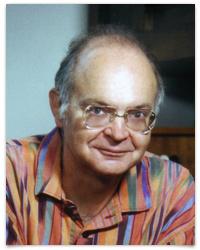
\includegraphics[scale=.5]{images/don_knuth.jpg}
\end{center}
	\caption{Don Knuth, the inventor of \TeX}
	\label{fig:sample}
\end{figure}

\section{Basic Terminology}
As usual the very basic terminology is briefly explained here. Most probably the explanations here only scratch a surface level. More detailed explanations of terminology goes into chapter~\ref{cha:theoretical-background}.

\section{Related Work and Projects}
Here a survey of other work in and around the area of the thesis is given. The reader shall see that the authors of the thesis know their field well and understand the developments there. Furthermore here is a good place to show what relevance the thesis in its field has.

\section{Structure of the Thesis}
%dsflkjas flaksjfl asdfj as lfjldsajflaksdjf sa dfjlasdkfj sadlfjasdklf als dfj l dfsdfsdfn chapter~\ref{cha:used-technologies} (\nameref{cha:used-technologies}) on page~\pageref{cha:used-technologies} we describe the used technologies.
Finally the reader is given a brief description what (s)he can expect in the thesis. Each chapter is introduced with a paragraph roughly describing its content.